%%===================Método proposto==============%%
\section{Método Proposto}
\subsection{Método Proposto}
\frame{
  \frametitle{Método Proposto}
   

      	\begin{itemize}
      	 \item Esta proposta visa a aplicação da EG para geração de heurísticas
      	 de alto nível para uma plataforma hiper-heurística para o PDP (HyPDP).
      	 \item Baseada no trabalho desenvolvido por Sabar et al. \cite{sabar2015automatic}.
      	 \item No contexto desta proposta:
      	   \begin{itemize}
	      	 \item Heurísticas de alto nível consistem de um \textbf{mecanismo de seleção} e um \textbf{critério de aceitação}. 
	      	 \item Heurísticas de baixo nível são compostas por um conjunto de heurísticas, selecionadas de
	      	 estudos anteriores, um mecanismo de memória e uma função de \textit{fitness}.
      	   \end{itemize}
      	\end{itemize}

}


\subsection{Método Proposto}
\frame{
	\frametitle{Método Proposto}

		\begin{figure}[!htb]
			\centering
			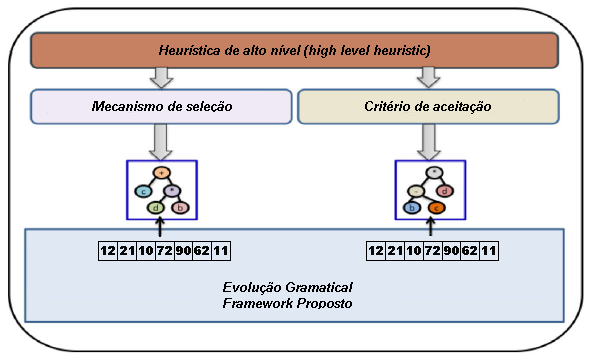
\includegraphics[scale=.8]{figuras/ProposedFramework.png}
			\caption{Método proposto}
			\label{fig:proposedFramework}
		\end{figure}	

}



\subsection{Gramática Proposta}
\frame{
	\frametitle{Gramática Proposta}

		\begin{figure}[!htb]
			\centering
			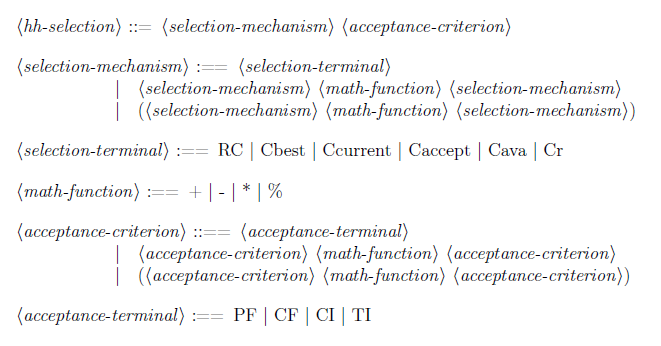
\includegraphics[scale=.6]{figuras/ProposedGramatica.png}
			\caption{Gramática para converter vetores de inteiros em heurísticas de alto nível.}
			\label{fig:proposedGrammar}
		\end{figure}
		

}


\subsection{Terminais para gerar mecanismos de seleção}
\frame{
	\frametitle{Terminais para gerar mecanismos de seleção}
	

		\begin{itemize}
			\item RC (\textit{Reward Credit}): Recompensa que uma determinada heurística de baixo nível deve receber baseado no seu desempenho. O cálculo da melhoria é dado por: $M(i) = (|f1 -f2|/f1) *100$ se $f2 < f1$, onde $f1$ é a qualidade da solução corrente e $f2$ é a qualidade da solução resultante. 
			A melhoria obtida é salva em uma janela deslizante (FIFO) de tamanho W. O crédito de qualquer heurística de baixo nível é então atribuído como o máximo valor na janela deslizante correspondente. 
			%A ideia por trás deste critério é: heurísticas de baixo nível que não são usadas com frequência mas que alteram a solução com grandes melhorias tendem a ter mais preferência do que aquelas que geram pequenas melhorias. Portanto as heurísticas que trazem frequentes, mas pequenas melhorias irão ter menos probabilidade de serem selecionadas.
			\item \textbf{$C_{best}$}: Número de vezes que a i-ésima heurística de baixo nível atualizou a melhor solução conhecida. Este critério favorece as heurísticas de baixo nível que obtiveram êxito em melhorar a melhor solução conhecida até o momento. Este critério é útil para sistematicamente melhorar o atual mínimo local.
		  
		\end{itemize} 
		
		

}


\subsection{Terminais para gerar mecanismos de seleção (cont.)}
\frame{
	\frametitle{Terminais para gerar mecanismos de seleção (cont.)}
	

		\begin{itemize}
			\item $C_{current}$: Número de vezes que a i-ésima heurística de baixo nível atualizou a solução atual. Este critério favorece as heurísticas de baixo nível que obtém êxito em atualizar a solução corrente. Este critério serve para deixar a busca concentrada próxima à solução corrente.
			\item $C_{accept}$: Número de vezes que a solução gerada pela i-ésima heurística de baixo nível foi aceita pelo critério de aceitação. Irá favorecer heurísticas de baixo nível que podem ajudar a escapar de um mínimo local.
			\item $C_{ava}$: A média de melhorias anteriores da i-ésima heurística de baixo nível. Este critério favorece heurísticas de baixo nível que realizaram grandes melhorias em média.
			\item $C_r$: O número de vezes que a i-ésima heurística de baixo nível foi classificada como primeira.
			
		\end{itemize} 
			

}


\subsection{Terminais para gerar critérios de aceitação}
\frame{
	\frametitle{Terminais para gerar critérios de aceitação}

	 \begin{itemize}
		 	\item Delta: A diferença da qualidade entre a solução corrente e a solução descendente.
		 	\item PF: A qualidade da solução anterior.
		 	\item CF: A qualidade da solução atual.
		 	\item CI: Iteração corrente.
		 	\item TI: Número de iterações.
	 \end{itemize}
		
		

}



\subsection{Funções matemáticas para gerar as heurísticas de alto nível}
\frame{
	\frametitle{Funções matemáticas para gerar as heurísticas de alto nível}

		 \begin{itemize}
		 	\item +: Adiciona as duas entradas.
		 	\item -: Subtrai a segunda entrada da primeira.
		 	\item *: Multiplica as duas entradas.
		 	\item \%: Divisão protegida, isto é, se o denominador for 0, o altera para 0,001.
		 \end{itemize}

}


\subsection{EG para gerar heurísticas de alto nível}
\frame{
	\frametitle{Método Proposto}
	

		\begin{itemize}
			\item Utilizando a gramática apresentada e vetores de inteiros é possível gerar heurísticas de alto
			nível. Os conjuntos terminais da gramática apresentam estatísticas sobre as heurísticas de
			baixo nível e estas são a matéria-prima para a construção dos componentes das heurísticas
			de alto nível para o HyPDP.
			
			\item O próximo passo consiste em evoluir uma população de vetores de inteiro, gerados de
			maneira aleatória, utilizando o processo evolutivo descrito anteriormente.
		\end{itemize}
		
		

}


\subsection{Função de fitness para a evolução gramatical}
\frame{
	\frametitle{Função de \textit{fitness} para a evolução gramatical}
	
			\begin{itemize}
			\item Uma função de \textit{fitness} baseada na função proposta por Sabar et al. \cite{sabar2015automatic} foi desenvolvida para esta proposta.
			
			\item A probabilidade de selecionar indivíduos é alterada de acordo com a qualidade
			da melhor solução retornada pela execução da plataforma  hiper-heurística HyPDP, utilizando
			o mecanismo de seleção e critério de aceitação.
			
			\item A
			qualidade retornada pela solução pode ser pior ou melhor do que a solução utilizada como
			entrada para a plataforma hiper-heurística.
		
			\end{itemize}
		
}


\subsection{Função de fitness para a evolução gramatical}
\frame{
	\frametitle{Função de fitness para a evolução gramatical}		

Suponha que $f_i$ e $f_b$ representem a qualidade da solução inicial e da retornada e $Ph[]$ o vetor de probabilidades de seleção dos indivíduos da EG. A retribuição para o $i-$ésimo indivíduo, caso tenha obtido uma melhoria, é calculada utilizando a equação \ref{eq:fitnessFunction1}.

	\begin{block}{Função de \textit{fitness} para retribuição ao $i-$ésimo indivíduo}
		
		 \begin{equation} {}
		 \label{eq:fitnessFunction1}
		 Ph[i] = Ph[i] + \sigma 
		 \end{equation}
		  Onde:
		 \begin{equation}
					 \sigma = (f_i - f_b)/(f_i + f_b). 
		 \end{equation}		
	\end{block}
}





\subsection{Função de fitness para a evolução gramatical}
\frame{
	\frametitle{Função de fitness para a evolução gramatical}		
	
	Os demais indivíduos diferente de $i$ devem receber uma penalização. Suponha que $Nh$ seja o número de indivíduos a penalização é calculada utilizando a equação \ref{eq:fitnessPenalizeFunction1}.
	\begin{block}{Função de \textit{fitness} para penalização aos outros indivíduos}
		\begin{equation} {}
		\label{eq:fitnessPenalizeFunction1}
		Ph[j] = Ph[j] - (\sigma / (Nh - 1))
		\end{equation}
		Tal que:	
		\begin{equation} {}
		\label{eq:fitnessPenalizeFunction2}
		j \in \{1, ..., Nh\} ~e~ j \neq i
		\end{equation}
		
	\end{block}
}	


\subsection{Função de fitness para a evolução gramatical}
\frame{
	\frametitle{Função de fitness para a evolução gramatical}		
	
	Caso contrário (se a solução retornada não for melhor que a utilizada como entrada), uma penalização é aplicada ao $i$-ésimo indivíduo utilizando a \autoref{eq:fitnessBadFunction1}.
	\begin{block}{}
		\begin{equation} {}
		\label{eq:fitnessBadFunction1}
		Ph[i] = Ph[i] - |\sigma \times \alpha|
		\end{equation}
		
		Onde: 
		\begin{center}
			$\alpha =$ iteração corrente $/$ número total de iterações.
		\end{center} 
	\end{block}
	
	
	
}	



\subsection{Objetivos}
\frame{
	\frametitle{Objetivos}
	
	\begin{block}{Objetivos do trabalho}
			\begin{itemize}
				\item Texto;
				\item Texto;
				\item Texto;
				\item Texto;
				\item Texto.
			\end{itemize}
	\end{block}
	
	\begin{block}{Funções objetivas do trabalho}
		\begin{itemize}
			\item $ maxf_{i}(T)=pc(T) $
			\item $ minf_{ii}(T)=\frac{custo(T)}{nº \; c \; de \; t} $
			\item $ maxf_{iii}(T)=\frac{pref(T)}{nº \; c \; de \; t} $
			\item $ maxf_{iv}(T)=escore(T) $
			\item $ minf_{v}(T)=nCasos(T) $
		\end{itemize}
	\end{block}
}

\frame{
	\frametitle{Funções objetivas do trabalho}
	
	\begin{block}{Funções objetivas do trabalho}
		\begin{itemize}
			\item $ pc(T)=\frac{(nº \; de \; p \; c)}{(nº \; de \; p \; c)}  $
			\item $ c(T)=\displaystyle\sum_{i=0}^{i<n} c(p_{i}) $
			\item $ p(T)=\displaystyle\sum_{i=0}^{i<n} p(p_{i}) $	
			\item $ score(T)=\frac{(nº \; de \; m \; m)}{(nº \; de \; m \; g + nº \; de \; m \; e)} $
			\item $ nCasos(T)=\frac{(nº \; de \; c \; de \; t)}{(total \; de \; p)}  $
		\end{itemize}
	\end{block}
}

\frame{
	\frametitle{\textit{Tabela}}

	\begin{block}{\textit{Tabelas} utilizadas}
	\begin{table}[!htb]
		\renewcommand{\arraystretch}{1.5}
		\fontsize{10pt}{12pt}\selectfont
		\centering
		\scalebox{0.8}{
			\begin{tabular}{c | c | c | c | c }
				\toprule
				\textbf{Matriz} & \textbf{Qtde de P} & \textbf{Qtde de M} & \textbf{Qtde de Pa} & \textbf{Qtde de C}\\ \midrule
				texto1 & 450 & 227 & 183 & 21\\ \midrule
				texto2 & 1152 & 394 & 202 & 22\\ \midrule
				texto3 & 68 & 106 & 75 & 14\\ \midrule
				texto4 & 504 & 357 & 195 & 22\\
				\bottomrule
			\end{tabular}
		}
	\end{table}
	\end{block}
}